\chapter{IMSI Catcher Detection}
\section{Framework and Hardware}
The following section will give an overview of the OsmocomBB framework and how it works in conjunction with the Motorola C123 mobile phone to enable information harvesting for the \gls{icds}.
OsmocomBB is one of many \gls{osmo} projects\footnote{Osmocom, \url{http://osmocom.org/} [Online; Accessed 04.2012]}. It implements the software part of a mobile phone.
Another project is OpenBSC which implements software for configuring and operating a \gls{bsc}.
OpenBSC was used to realise the Open Source IMSI Catcher \cite{dennis} and the base station that will be used later to evaluate the performance of the \gls{icds}.

\subsection{OsmocomBB}
OscmocomBB implements the baseband part of \gls{gsm} as an open source project.
Baseband part in this case means that it is an open source software to control the baseband chip inside the mobile phone.
The goal is to have, by using compatible hardware, a phone using free software only as opposed proprietary baseband implementations.
Therefor the project scope is implementing \gls{gsm} layer 1-3 as well as hardware drivers for the baseband chipset.
A simple user interface on the phone is planned but not yet implemented.
At this stage a verbose user interface on the computer is used.
This could be beneficial to multiple areas \cite{osmo_rationale}:
\begin{itemize}
	\item \textbf{Security:} The software running on the baseband chips is highly proprietary and closed.
	The source is often disclosed only to the mobile phone manufacturers using the specific chipset.
	One cannot be sure that this software does not have bugs that could be exploited and ultimately pose a security risk to the subscriber.
	History has shown that open source projects are more secure than proprietary solutions since more people can view the source to find issues.
	If a security threat is found the bug is fixed fast and a patch is released.
	This could be a great benefit for phone users.
	\item \textbf{Education:} Currently knowledge about \gls{gsm} and its layers on a technical level is not very well spread.
	An open source implementation as a reference could serve to educate more developers generally interested in the subject of mobile communications and thus improve products and software.
	Additionally this implementation enables universities to hold practical lab courses and interested individuals to do hands-on experiments.
	\item \textbf{Research:} A free implementation can decouple research on \gls{gsm} technologies from the industry since key technologies are no longer only available to researchers employed by a specific company.
	Additionally this way security holes can be uncovered more easily.
	Modifications to the protocol stack can be deployed and tested in a real environment.
\end{itemize}

\subsubsection{Project Status}
At this point layer two and three do not actually run on the phone but rather on a computer to which the phone is connected via a serial cable
Layer 1 runs inside the custom firmware on the \gls{me} itself, since the procedures involving layer 1 are time critical.
This has advantages as well as disadvantages.
The disadvantage is that in order to run an application written with OsmocomBB you always have to have a notebook in addition to the phone.
The benefit however is that during the development process, the phone does not have to be touched after an initial deployment of the firmware.
This means code can be modified, compiled and tested locally without the need of remote debugging.
Experimenting is considerably easier this way.
This separation however would not work in the original \gls{gsm} specification, therefore an extra interface layer between layer 1 and 2 had to be implemented to handle messaging between those two.
It is called Layer 1 Control, L1CTL.

The current state of the project is, according to a presentation given on the 27$^\text{th}$ chaos communication congress\footnote{27C3 public wiki (Day 3), \url{http://events.ccc.de/congress/2010/wiki/Welcome} [Online; Accessed 04.2012]} by Dieter Spaar and Harald Welte, that the network layers 1-3 are fully implemented, SIM cards can be accessed or emulated and \gls{gsm} cell selection and reselection are working.
A3/A8 as well as A5/1 and A/52, Full Rate and Enhanced Full Rate codecs are there, so it is possible to do voice calls with an OsmocomBB application written for that purpose, called \texttt{mobile}.
It features a terminal/telnet based interface much like Cisco routers however there is no user interface for the phone so far or any implementation for Handovers since neighbourhood measurements were not implemented in the framework at that point.
During these calls or during the operation of other programs, it is possible to receive all the frames that are being transmitted via Wireshark from the \texttt{osmocon} application.

\subsection{Motorola C123}
\label{sec:osmo_phones}
Since the general idea behind OsmocomBB was to become a vendor independent open source \gls{gsm} implementation for everyone to use, there were certain requirements the targeted hardware would have to meet.
For the consumer side requirements these were having a low price and a good availability.
This criterion rules out \gls{diy} approaches since the number of produced devices would be low and thus costly or a significant technical knowledge would be expected from all users to assemble the hardware.
For the developer side this would also mean implementing a lot on the lower levels of analog logic.
Therefore the Motorola C123 was chosen, an old, very cheap phone that is well spread.
It has the advantage of being very simple on the hardware side since it is based on the well documented Texas Instruments Calypso Chipset \cite{osmo_slides}.
Table \ref{tab:c123_specs} shows an overview of the main specifications for the phone.
\begin{table}
\centering
	\begin{tabular}{ll}
	\toprule
	Component			&Specification\\
	\midrule
	Band 				&GSM 900, GSM 1800\\
	Size				&$101\times 45\times 21$ mm\\
	Weight				&86 g\\
	Battery				&920mAh Li-Ion battery\\
	Digital Baseband	&Texas Instruments Calypso\\
	Analog Basenand		&Texas Instruments Iota TWL3025\\
	GSM Transceiver		&Texas Instruments Rita TRF6151C\\
	\bottomrule
	\end{tabular}
	\caption{Technical specifications for the Motorola C123.}
	\label{tab:c123_specs}
\end{table}
The OsmocomBB framework should work well or with small adjustments for any phone that share the same components.
Figure \ref{fig:osmo_c123} an image of the Motorola C123 circuit board with the components mentioned before.
\begin{figure}
\centering
	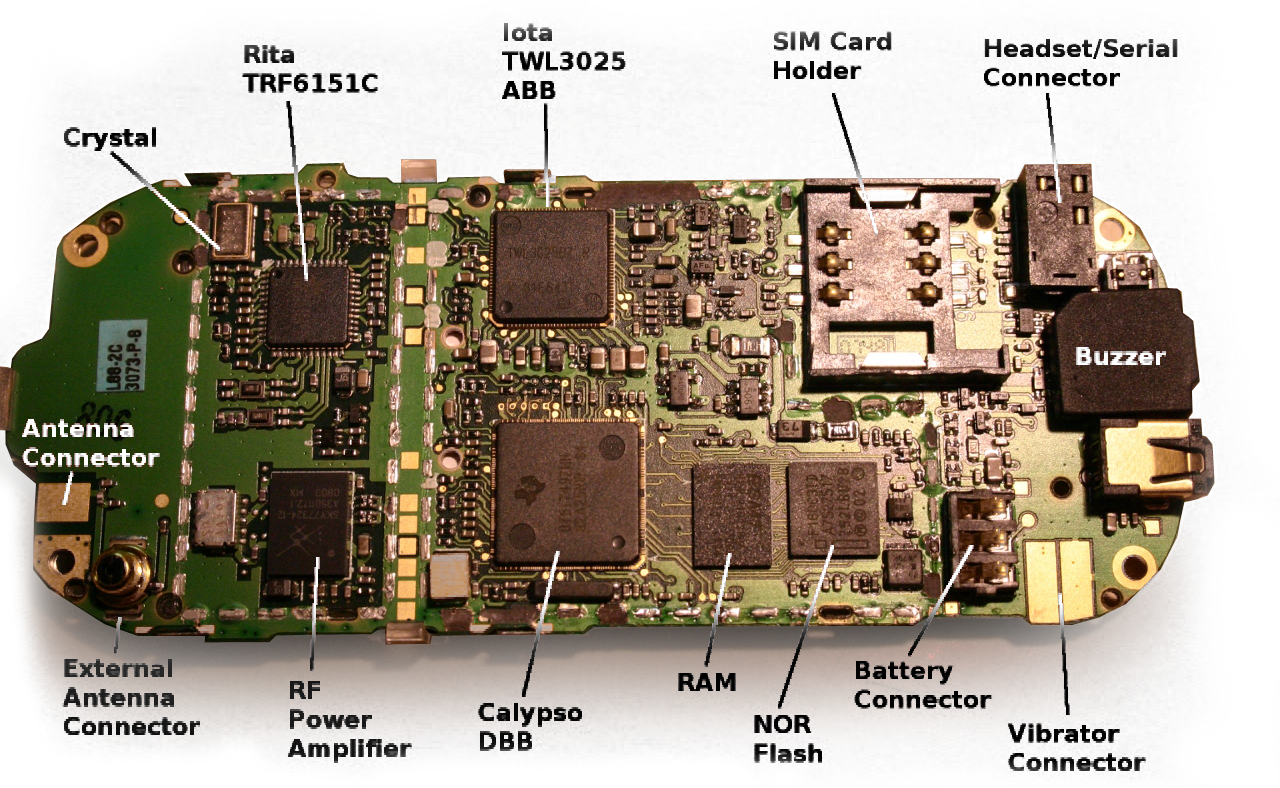
\includegraphics[width=.9\textwidth]{../Images/c123_pcb}
	\caption{Circuit board of the Motorola C123 with its components \cite{osmo_wiki_c123}.}
	\label{fig:osmo_c123}
\end{figure}
Another reason for choosing this hardware platform was that during the start of the OsmocomBB project an open source implementation of \gls{gsm} layer 1 was already available on Sourceforge (TSM30 Project) that could be used as a reference. 
At this point the original project has been removed from the Sourceforge site.

In order to use the Motorola C123 in combination with the OsmocomBB framework the custom firmware implementing layer 1 and L1CTL has to be flashed onto the board.
This has to be done using a RS332 serial cable that is connected to the 2.5\,mm audio jack.
The audio jack of the Motorola C123 and other Calypso based mobile phones typically have a 3.3 V serial port on their audio jacks.
These cables are normally referred to as T191 unlock cables 
A variety of stores around the internet sell the cables ready made for about \$10-\$15\footnote{FoneFunShop, \url{http://www.fonefunshop.co.uk/cable_picker/773_Motorola_T191_W220_W375_OSMOCOM_etc._USB_Unlock_Cable.html} [Online; Accessed 04.2012]}.
One must be careful when using the PC's serial port to communicate with the phone though.
Since the phone's serial operates at 3.3\,V and is internally connected to the 2.8\,V IO-pins of the baseband processor, directly connecting it to the computers 12\,V serial port will destroy the hardware.
Therefore it is recommended to use a USB serial cable.
Schematics for such an unlock cable, along with a few instructions on how to build one are given in Appendix \ref{sec:osmo_serial_schematics}.

Another issue is virtualisation.
The bootloader and the firmware can fail to be deployed correctly if a virtual machine is used as development system.
This is because the protocol used by Motorola to do the actual flashing process is \emph{very} time critical and thus timeouts can occur that are caused by the overhead the virtual machine imposes on the hardware/software communication.

\subsection{OsmocomBB and ICDS}
The setup that is used for the \gls{icds} project can be seen in Figure \ref{fig:osmo_setup}.
It was build and tested in a Xubuntu 11.10 environment \footnote{Xubuntu, \url{http://xubuntu.org/} [Online; Accessed 04.2012]} which is a more lightweight variant of the popular Debian based Ubuntu Linux distribution.
The process of acquiring, compiling and running the OsmocomBB framework itself in this environment is explained in Appendix \ref{sec:osmo_install}.
As can be seen in the diagram, layer 1 of the OsmocomBB \gls{gsm} stack runs on the phone.
It is connected via a serial cable to the computer running the \gls{icds}.
On the computer side the \texttt{osmocon} program provides a general interface to the phone.
\texttt{Osmocon} is also used to download the firmware to the Motorola C123.
Other software can communicate with \texttt{osmocon} and subsequently with the phone using unix sockets.
\begin{figure}
\centering
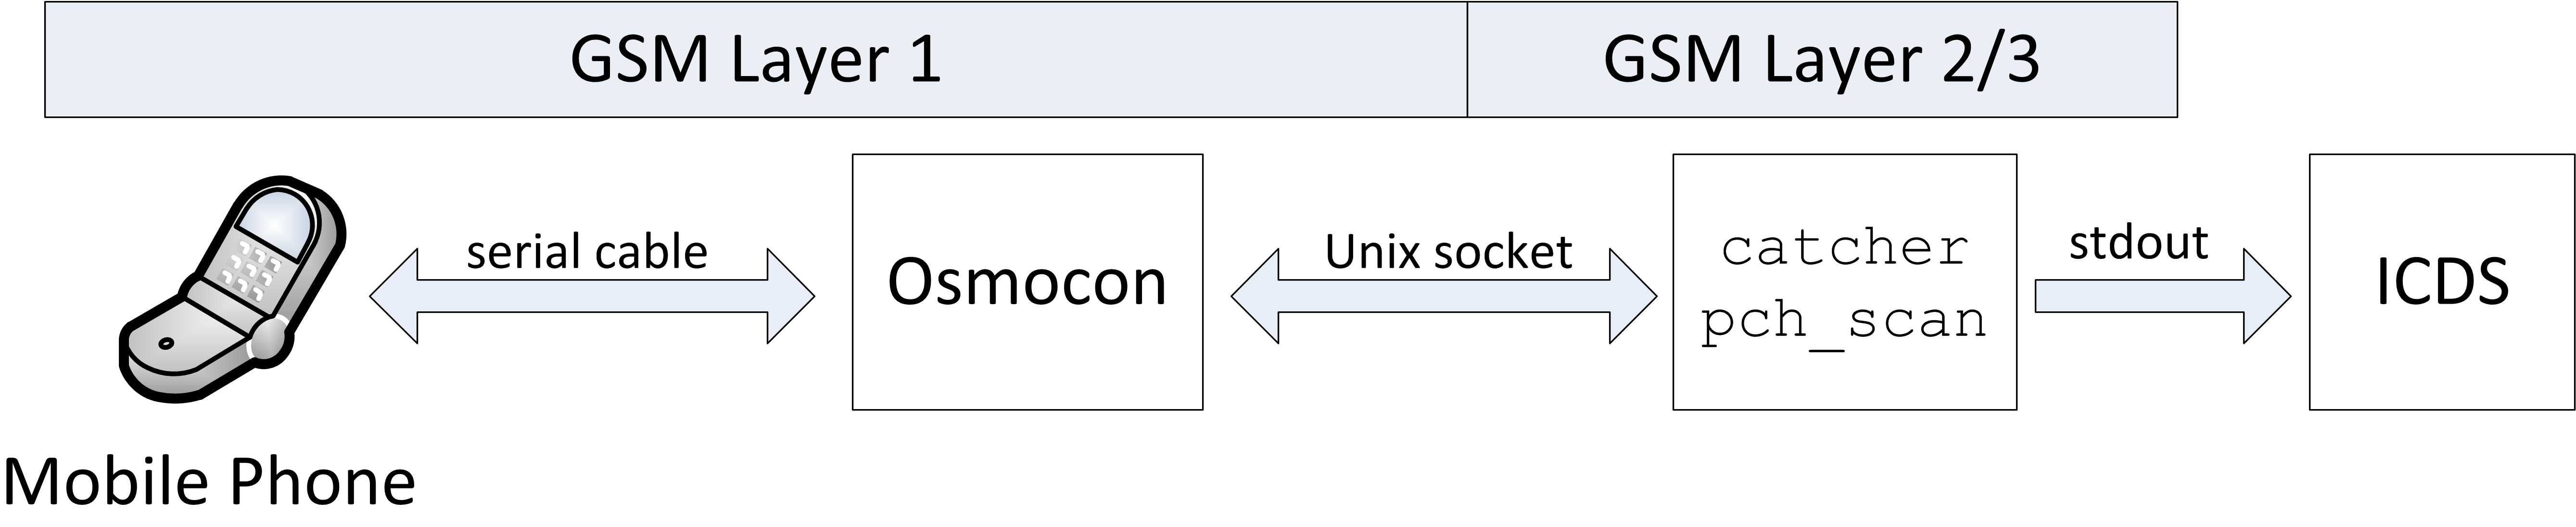
\includegraphics{../Images/OsmoStructure}
\caption{Interaction of the OsmocomBB components with the ICDS software.}
\label{fig:osmo_setup}
\end{figure}

\texttt{Catcher} is a modified version of the \texttt{cell\_log} program by Andreas Eversberg that interfaces with \texttt{osmocon} to harvest information from \glspl{bts} and forward it to the \gls{icds}.
It can be seen as a layer 3 program that scans through available frequencies and reads information from the \gls{bcch} whenever one such channel is available on the frequency at hand.
The forwarding is done directly via \texttt{stdout} since it runs as a child process of the \gls{icds}.
The functionality of \texttt{catcher} will be explained in detail in Section \ref{sec:info_gathering} while the implementation and operation of the \gls{icds} will be discussed in Section \ref{sec:icds}.

\section{Procedure}
The main goal of the \gls{icds} is to reach a conclusion on whether it is safe to initiate a phone call or not, in other words if the base station our mobile phone will connect to is trustworthy.
As mentioned before as soon as a subscriber connects to an IMSI Catcher it automatically gives up information on his/her location.
Therefore this project will use a passive approach on information harvesting, meaning we will only use information that is broadcasted or freely available as to not give up any hints of the \gls{icds} being active.

To that end a four-step process is taken.
First the information is gathered.
This process is explained in detail in Section \ref{sec:info_gathering}.
After information on the surrounding \glspl{bts} is ready in the \gls{icds}, a set of checks is evaluated on each base station individually, with each yielding a specific result for the station.
These checks are called \emph{rules} and discussed further along with the next two steps in Section \ref{sec:info_evaluation}.
Afterwards the results the rules yielded for each base station have to be aggregated into one single result for each \gls{bts}.
At last, after every \gls{bts} has its evaluation it can be decided whether to tell the subscriber it is safe to initiate a phone call or not.

\subsection{Information Gathering}
\label{sec:info_gathering}
As explained in Section \ref{sec:common_channels} every base station has an associated \gls{bcch} where information about the station and its network is spread.
\gls{bcch} frames are always sent inside a 51-Multiframe.
After the \gls{ms} has synchronised using the values on the \gls{fcch} and \gls{sch} it can determine which kind of information is hosted inside the \gls{bcch} message.
These so called System Information Messages originate at the \gls{bsc} and are produced for each \gls{bts} individually and then periodically broadcasted.
Since all the required information would not fit inside a single frame there are different kinds of System Information Messages that are distinguished by their \gls{tc} and host different kinds of information.
The type can be extracted using the \gls{fn} of the frame the message is sent in \cite{GSM2009}:
\[\text{TC}=(\text{FN} \text{ div } 51)\text{ mod } 8\]
Table \ref{tab:tc_mapping} shows how the \glspl{tc} can be mapped on those types.
\begin{table}
\centering
\begin{tabular}{lc}
\toprule
TC		&System Information Type\\
\midrule
0		&Type 1\\
1		&Type 2\\
2,6		&Type 3\\
3,7		&Type 4\\
4,5		&Any (optional)\\
\bottomrule
\end{tabular}
\caption{Type Codes and the corresponding System Information Types \cite{GSM2009}.}
\label{tab:tc_mapping}
\end{table}
For this project the System Information Type 1-4 are of interest because these are available to all \glspl{ms} that tune in to the particular \gls{bcch} of the respective \gls{bts} without actively connecting to it.

The information contained inside the System Information Messages is harvested via the \texttt{catcher} program.
\texttt{Catcher} is implemented inside the OsmocomBB framework and connects over the \texttt{osmocon} application to the Motorola C123.
At first a sweep scan is done over all the \glspl{arfcn} to measure their reception levels in order to determine where base stations and thus \glspl{bcch} are located.
Afterwards \texttt{catcher} tunes the phone to those specific frequencies where a \gls{bts} was found 

At each such frequency it waits until all the System Information Messages are gathered and extracts parameters where possible.
The parameters along with the raw data are forwarded to the main \gls{icds} application for further evaluation.
An example of a fully parsed System Information Type 1 can be seen in Figure \ref{fig:si1} \cite{protocols1999}.
\begin{figure}
\centering
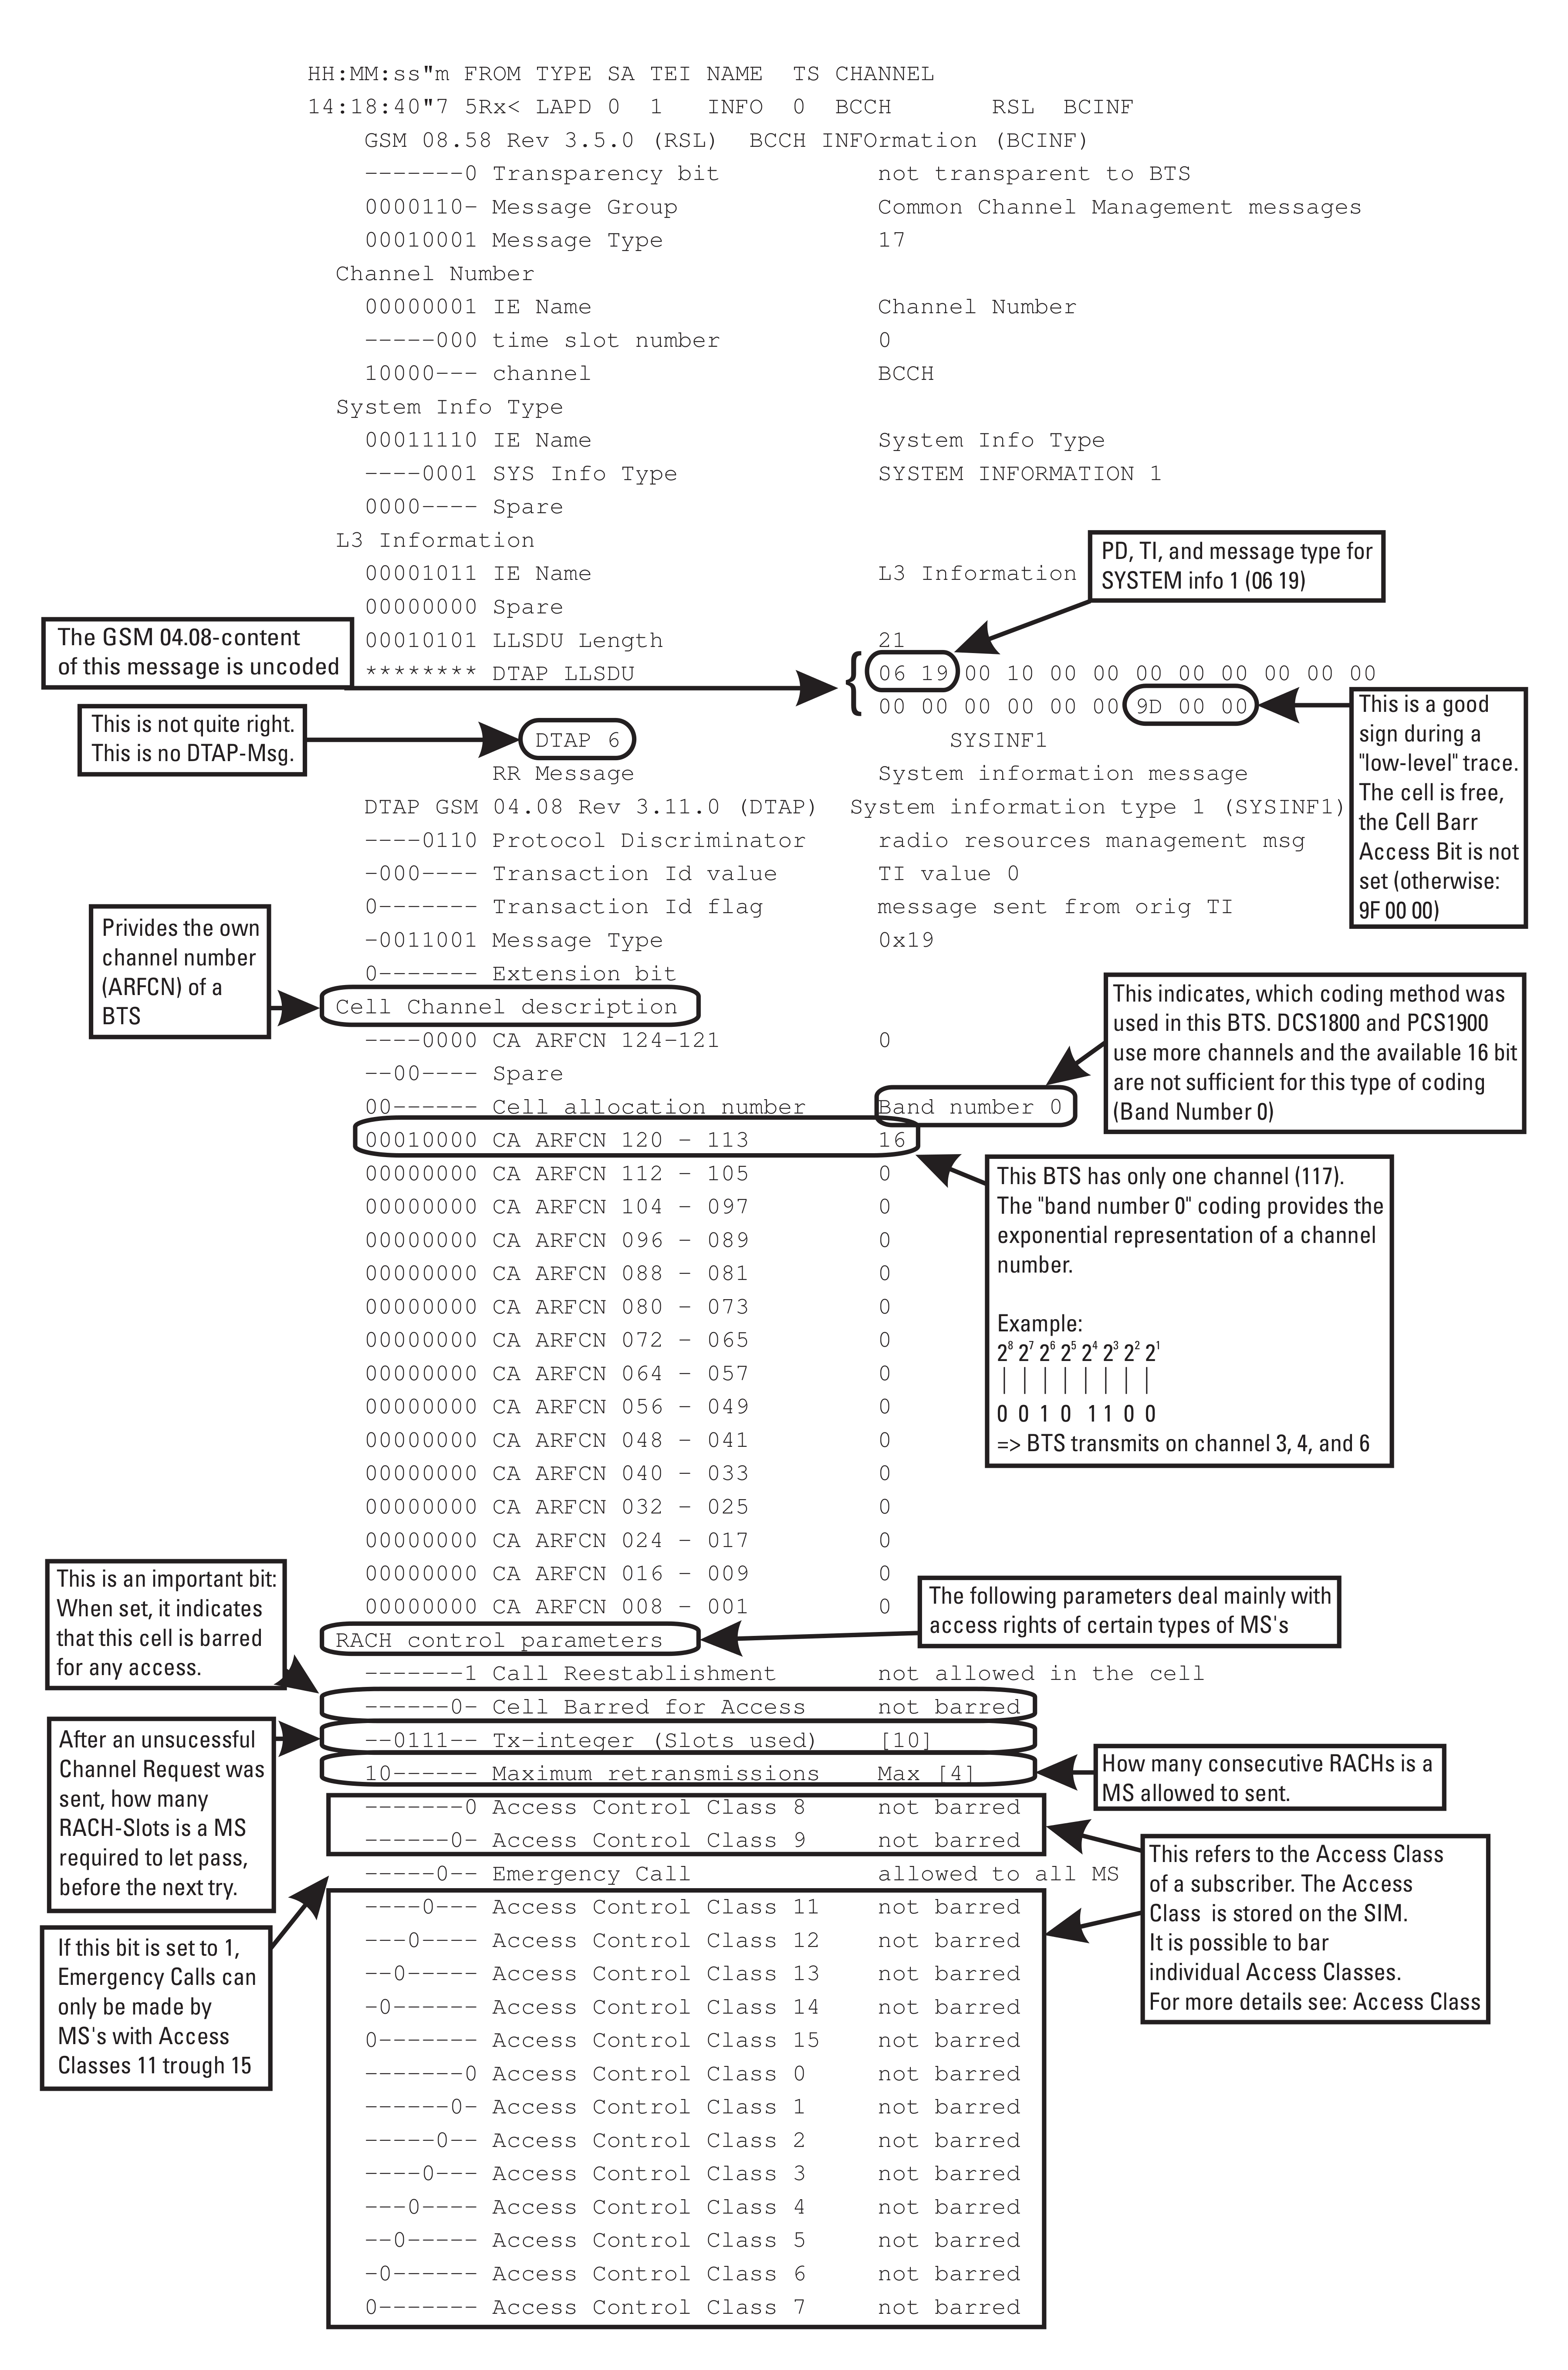
\includegraphics[width=.9\textwidth]{../Images/sysinfo1}
\caption{System Information 1 Message \cite{protocols1999}.}
\label{fig:si1}
\end{figure}
Examples for all the System Information Messages used, along with an interpretation are located in Appendix \ref{sec:system_infos}.
As long as scanning mode is active all the available stations are scanned repeatedly and changes in the \glspl{bts} will continuously update the data model inside the \gls{icds} software.
The parameters harvested are:
\begin{itemize}
	\item Country: The interpreted country code the base station is broadcasting.
	\item Provider: The interpreted provider code the base station is broadcasting.
	\item ARFCN: The \gls{arfcn} on which the base station is located.
	\item rxlev: Receiving strength in db.
	This parameter is measured by the Motorola C123 and not part of the System Information Messages.
	Even small changes in the location can have a large impact on this parameter due to shadowing and reflection.
	However it can be used in certain cases as will be discussed in Section \ref{sec:fake_parameters}.
	\item BSIC: Because of frequency reuse in a cellular network it is possible that two different base stations can sent at the same \gls{arfcn}.
	In order for the \gls{ms} to keep these apart the \gls{bsic} is also broadcasted.
	It consists of a \gls{ncc} identifying the provider, so the \gls{ms} can filter out messages that it does not need beforehand and the \gls{bcc} that must be unique for a given provider over all base station in a large area.
	\item LAC: This is the last part of the \gls{lai} (that consists of \gls{mcc} + \gls{mnc} + \gls{lac}) and is a hierarchical identifier for a given base station.
	The hierarchy is provider wide, meaning two different providers may use \glspl{lac} with a completely different numbering system.
	The \gls{lac} is used by the provider to tell the \gls{me} that it entered a new area and has to announce itself.
	\item Cell ID: The Cell ID is a globally unique identifier for the cell the \gls{ms} is connected to.
	\item Neighbouring Cells: Each base station keeps a list of other base stations in the perimeter  for the \gls{ms} to scan and determine if there is a \gls{bts} with a better reception in the area.
	\item Encryption: The encryption algorithm used to encrypt the voice data.
\end{itemize}
Note that there are different formats for the Neighbouring Cell List since the original number of 17 bytes could only present a bit mask for 124 neighbouring \glspl{arfcn}.
This works for the 900 MHz band, but for the extended 900\MHz and the 1800\MHz band the System Information Type 2bis and System Information Type 2ter have to be harvested additionally to construct the Neighbouring Cell List.

%TODO:finish encryption
Encryption cannot actually be read passively from a base station since the encryption algorithm is determined when a connection is established (finish paragraph on encryption when feature is finished).

\subsection{Information Evaluation}
\label{sec:info_evaluation}
Each base station is evaluated the moment the data completely arrived at the \gls{icds} application.
Additionally when a new \gls{bts} has been found and added all formerly discovered stations are also re-evaluated since new discoveries can have an impact on the rules that evaluate the context surrounding an old base station.

As mentioned above, evaluation is done based on constructs called rules.
Each rule represents one check that can be performed on a base station and yields a result based on its findings.
A \emph{Critical} result means that the base station evaluated has a critical configuration error or critical settings that are not found on normal base stations, \eg unknown provider names or encryption that is turned off.
This station should not be trusted.

If  a \emph{Warning} status is yielded the \gls{bts} at hand has some concerning features but it could not be said whether it really is an IMSI catcher or sheer coincidence.
An example would be a base station having a  neighbouring cell list of which none of the cells therein have actually been found up to that point.
The list could either be a fake or it could simply be coincidence that the scan has not found any.
They could have been out of range for example.

In some cases a rule cannot yield a finding.
That is when the state is explicitly set to \emph{Ignore} so the evaluator knows that this rule should have no influence on the final outcome.	
This is the case for example when trying to find whether the base station uses encryption or not and no other subscriber connects until a set timeout is reached.

If everything went as expected, \emph{Ok} is returned.

These rules can be divided into two different categories depending on how they work and which situations they are tailored to.
Most of the rules are parametrised so they can be tweaked to different environments and standards.

The first set of rules called \emph{Configuration Rules} targets the base station itself.
Rules in this category are meant to check parameters that concern the \gls{bts} for integrity and configuration mistakes that could have been made by an IMSI catcher operator.
An overview of which Configuration Rules are currently implemented inside the \gls{icds} is given in Table \ref{tab:config_rules}.
\begin{table}
\centering
\begin{tabular}{ll}
\toprule
Rule					&Functionality\\
\midrule
Provider Known			&Checks whether the provider is in a list of known \\
						&providers.\\
Country/Provider Map	&Checks whether the given provider is a valid provider\\
						&for the given country.\\
LAC/Provider Map		&Checks whether the LAC of the station is in the normal\\
						&LAC range for that provider given the area.\\
ARFCN/Provider Map		&Checks whether the ARFCN is in the officially registered\\
						&range of the provider.\\
Encryption Algorithm	&Checks which encryption algorithm is used.\\
\bottomrule
\end{tabular}
\caption{Configuration Rules implemented inside the ICDS.}
\label{tab:config_rules}
\end{table}
Since there is no official listing or rule how the \gls{lac} is derived the LAC/Provider Mapping Rule needs knowledge of the area in which the \gls{icds} is used.
The \gls{icds} itself can be used to gather that knowledge but it has to be done prior to using the rule for base station evaluation. 
The \gls{arfcn} range each provider has registered in Germany can be looked up at the website of the Bundesnetzagentur\footnote{Bundesnetzagentur Vergabeverfahren, \url{http://www.bundesnetzagentur.de/cln_1911/DE/Sachgebiete/Telekommunikation/RegulierungTelekommunikation/Frequenzordnung/OeffentlicherMobilfunk/VergabeVerfahrenDrahtlosNetzzugang/vergabeVerfahrenDrahtlosNetzzugang_node.html} [Online, Accessed 04.2012]} which is needed for the ARFCN /Provider Mapping Rule.

The second set of rules is called \emph{Context Rules}.
As the name suggests these rules serve the purpose of checking how well a given \gls{bts} fits into its neighbourhood.
Table \ref{tab:context_rules} shows which rules have been implemented.
The Neighbourhood Structure Rule will be explained in a bit more detail in the next section.
\begin{table}
\centering
\begin{tabular}{ll}
\toprule
Rule					&Functionality\\
\midrule
LAC Median Deviation	&Checks whether the LAC of the given BTS deviates\\
						&more than a certain threshold from the median LAC of\\
						&that provider.\\
Pure Neighbourhoods		&Checks whether all found stations in the Neighbouring\\
						&Cell List share the same provider.\\
Neighbourhood Structure	&Checks the structure of the Neighbouring Cell List for\\
						&certain patterns.\\
Fully Discovered Nbhds. &Checks whether all the cells in the Neighbouring Cell\\
						&List have actually been found.\\
Cell ID Uniqueness 		&Checks whether there are other cells with the same\\
						&Cell ID.\\
LAC Change 				&Checks whether the LAC changes in the course of a scan\\
rx Change				&Checks whether the reception level changed significantly\\
						&during the course of a scan\\
\bottomrule
\end{tabular}
\caption{Context Rules implemented inside the ICDS.}
\label{tab:context_rules}
\end{table}
For the LAC the median was chosen over the average since if an extreme value (ill configured IMSI catcher) exists it would have a too strong impact on the average to which all the \gls{bts} are compared.
It could even have such a strong effect on the average that legitimate base stations would fall below the threshold and be recognised as catchers.

\subsubsection{Neighbourhood Structure}
The neighbourhood structure is the graph that is described by the Neighbouring Cell List located in the System Inforamtion 2/bis/ter constructs.
Figure \ref{fig:neighbourhood_example} shows an example of the neighbourhood graphs at the Technische Fakult\"at of the University of Freiburg\footnote{Georges Koehler Allee, Freiburg}.
\begin{figure}
\centering
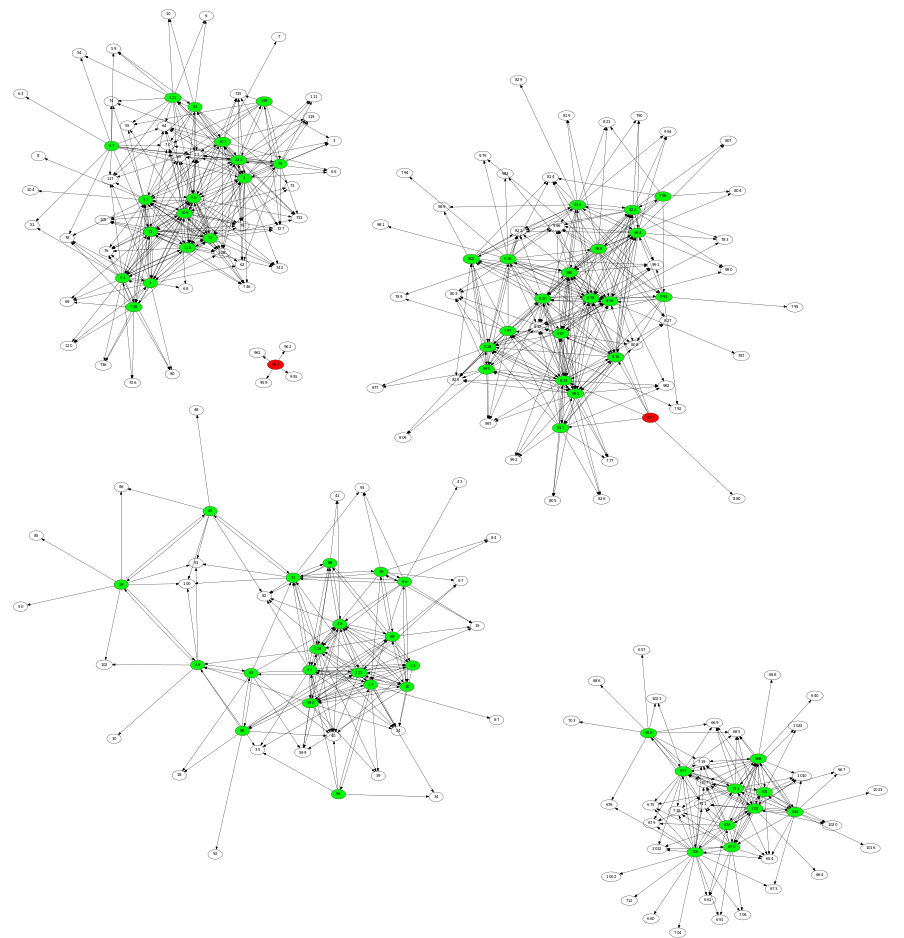
\includegraphics[width=.9\textwidth]{../Images/neighbourhoods_fak}
\caption{Base stations and their neighbourhood connections at the Technische Fakult\"at.}
\label{fig:neighbourhood_example}
\end{figure}
It can be seen that for each provider, the neighbourhood forms an isolated, nearly fully connected subgraph.
The bordering white nodes have not yet been discovered therefore they have no outgoing edges.
This could be the case because they are too far away for the Motorola to receive or because of signal damping due to shadowing and reflection effects.
In the \gls{icds} the aspect of isolated subgraphs for neighbourhoods is captured inside the \emph{Pure Neighbourhoods Rule}.
An interesting fact is that one node inside the E-Plus subgraph on the upper right is marked red.
This is because it is the \gls{bts} of the universities own \gls{gsm} network.
It was set up to be in a E-Plus neighbourhood but is not consistent with the E-Plus nodes surrounding it.
Therefore it is marked by the \gls{icds}.

Some of the attacks discussed in Section \ref{sec:attacks} imply a certain structure of the neighbourhood graph.
Since the IMSI catcher tries keep \glspl{ms} that have connected from switching back to a normal cell the neighbourhood list of such a catcher cell would either be empty or would only host neighbour cells that have a lower reception than itself.
An empty neighbourhood list is represented in the graph by a node that has been discovered and has no outgoing edges.
\begin{figure}
\centering
\subfigure[Normal neighbourhood]{
\begin{tikzpicture}[->,>=stealth',shorten >=1pt,auto,node distance=3cm,
  thick,main node/.style={circle,fill=blue!10,draw,font=\sffamily\Large\bfseries}]

  \node[main node] (1) {A};
  \node[main node] (2) [below left of=1] {B};
  \node[main node] (3) [below right of=1] {C};

  \path[every node/.style={font=\sffamily\small}]
    (1) edge  node {} (2)
        edge  node {} (3)
    (2) edge  node {} (1)
    	edge  node {} (3)
    (3) edge  node {} (1)
    	edge  node {} (2);
\end{tikzpicture}
}
\subfigure[Tainted neighbourhood]{
\begin{tikzpicture}[->,>=stealth',shorten >=1pt,auto,node distance=3cm,
  thick,main node/.style={circle,fill=blue!10,draw,font=\sffamily\Large\bfseries}]

  \node[main node] (1) {A};
  \node[main node] (2) [below left of=1] {B};
  \node[main node] (3) [below right of=1] {C};
  \node[main node] (4) [right of=1] {D};

  \path[every node/.style={font=\sffamily\small}]
    (1) edge  node {} (2)
        edge  node {} (3)
    (2) edge  node {} (1)
    	edge  node {} (3)
    (4) edge  node {} (1)
    	edge  node {} (2);
\end{tikzpicture}
}
\caption{Comparison between a normal neighbourhood subgraph and a tainted one.}
\label{fig:structure_comparison}
\end{figure}
Figure \ref{fig:structure_comparison} shows a simplified regular neighbourhood graph compared to a graph with two catcher nodes inside.
In this case catcher C chose the attack where it replaces a previously existent \gls{bts} whereas catcher D opened up a new cell.
Replacing has several advantages, one being already integrated in the neighbourhood of other nodes and thus being able to catch subscribers by handover.
For catcher D it is the other way around, it has only outgoing edges.
This means that this cell is not known by any other node of the same provider (of course the catchers provider is fake!).
Nevertheless it has some outgoing edges to nodes with significantly less transmission strength to not stick out too much as a completely isolated node.
Combinations of these two approaches are also possible.
These thoughts are basically what is captured inside the \emph{Neighbourhood Structure Rule}.

\subsubsection{Base Station Evaluation}
As mentioned at the beginning, all the rules are evaluated for each base station.
Aggregation of these rule results into a single result is done by modules called \emph{Evaluators}.
Currently there are three different evaluators implemented inside the \gls{icds}, with varying degrees of customisability.
\begin{itemize}
	\item Conservative Evaluator: This is a worst-case evaluator.
	It iterates over all the rule findings and yields the most concerning finding as its result.
	By default this evaluator is enabled in the system.
	\item Weighted Evaluator: Using this evaluator the user can give a weight to each rule.
	This way rules that are more important to the user can have a higher impact on overall evaluation.
	\item Grouped Evaluator: With this evaluator rules can be grouped together.
	Inside each group the result for the group is found by majority vote whereas the final result is conservatively found by comparing all the group results.
\end{itemize}
The different kinds of evaluators can be used to tweak the whole system more to a specific environment or purpose, if specific rules or groups of rules are given more weight.
After a finding has been determined for each station, all the results are again aggregated into a final result.
The overall result depends on which mode the \gls{icds} is used it.
If it is used as analysis tool the final result will be a conservatively aggregated result over all the stations in the list.
If the \gls{icds} is run in user mode, which is the mode an end user would use the system, the \gls{icds} looks up the provider the user has provided, filter out the base station with the best reception for that provider and yield its evaluation as final evaluation.
This reflects the fact that a subscriber cannot choose the \gls{bts} it connects to but the \gls{me} will rather connect to the best base station available for its given provider.

\subsection{Forged Parameters}
\label{sec:fake_parameters}
All of the parameters that have been looked at in this project so far are parameters that can directly be set by the operator of the \gls{bts} or IMSI catcher.
This is a major problem since how can an IMSI catcher be found that sends exactly the same information as a regular base station?
To further investigate this issue we will analyse based on the three attack types presented in Section \ref{sec:attacks} which parameters can be forged and which cannot.

For all three attack types presented it is possible to find a parameter configuration that does not raise suspicion, if the operator chooses a compatible \gls{arfcn}, \etc for the mimicked provider. 
However if the IMSI catcher does not have a different \gls{lac} it will not notice that a subscriber has just connected to it, as long as the subscriber stays passive.

The Neighbouring Cell List is a bit different.
Since the catcher wants to keep lured subscribers it will normally have an empty list or a list pointing only to \glspl{bts} that have a lower reception level. 
Both of these cases can be detected.
However the operator \emph{may} also choose to set a list consistent with the neighbouring cells.
This would lower the chances of success for the catcher but also make it blend better in its environment and thus harder to detect.

A sure criterion is the absence of an encryption algorithm which is needed by the catcher to record and monitor phone calls.
The main problem here is that it cannot be guaranteed that this parameter can be harvested.
Since this is a semi passive approach to harvesting it needs another subscriber to connect to the base station in question during the time the \gls{icds} is scanning it.
Also if the IMSI catcher is only set up to do localisation, the encryption can be enabled.

For the Cell ID there are basically two possibilities depending on which attack is used.
The first possibility is that the IMSI catcher replaces a formerly existent cell and the second one is that it opens up a new cell.
In the second case parameters can be chosen in a consistent way although a new Cell ID has to be chosen, as the Cell ID needs to be unique.
In the first case all parameters can be copied from the original cell.
Both possibilities can be resolved by adding outside knowledge to the \gls{icds} thus circumventing the problem of other parameters being forged.
This is done by rules called \emph{Database Rules}.

\subsubsection{Database Rules}
There are to different rules that each handles one of these cases.
The first case is the easier of both.
We know that the catcher cell has a new Cell ID that has not been there before.
Therefore the \emph{Cell ID Databse Rule} has two different means to exploit this fact:
\begin{itemize}
	\item A database of Cell IDs can be learned by the \gls{icds} beforehand. 
	This can be used to detect new Cell IDs that have not been seen before.
	\item A commercial Cell ID databse can be used to compare against the Cell IDs found by the \gls{icds}.
	A web service also offered by most providers of Cell ID databases.
\end{itemize}
The three largest Cell ID databases are the two commercial ones by Ericson\footnote{Ericson Labs, \url{https://labs.ericsson.com/apis/mobile-location/} [Online; Accessed 04.2012]} and combain\footnote{Mobile Positioning Solutions, \url{http://location-api.com/} [Online; Accessed 04.2012]} as well as the free alternative OpenCellID\footnote{OpenCellID, \url{http://www.opencellid.org/} [Online; Accessed 04.2012]} \cite{wiki_cells}.
Ericson and combain have trial modes, where the first 1000 requests are free for developers afterwards a subscription or a fee per request must be paid.
Another free alternative with a large coverage is Google Mobile Maps, that also offers a web service where CellIDs and their respecitve \glspl{lai} can be checked against their database to obtain localisation information (or simply check if they are part of the database).
By adding this information new cells can be identified.

The second where an existing cell is replaced is a bit more complicated since its parameters are an exact copy of the old cell.
Attacking by replacing a cell works in a way that the cell with the worst reception is targeted.
That way when the IMSI catcher finished replacing it, the reception goes up a significant amount and the mobile phone will initiate a handover to that cell.
The difference in reception can be used to identify this kind of attack.
In general the reception cannot be well used as a parameter because shadowing and reflection can substantially change the reception from one moment to the other.
However when reception intervals are logged for a fixed location like an office and important calls made from that specific location can be protected against this kind of attack.
To that end the \gls{icds} can monitor reception levels to build up databases with information about the reception intervals of the particular cells in different locations.
The\emph{Location Area Databse Rule} then checks if reception levels differ significantly for a given location.
If no database has been build beforehand but the \gls{icds} is stationary the \emph{rx Level Rule} can watch the reception level during the course of a scan and ensure that no change occured suddenly.

\subsubsection{Remaining Issues and Paging}
At this stage, if local information is given an IMSI catcher should be identified with a high probability.
However some issues still remain.
If a catcher is configured in a consistent way, replaces a cell and by chance has an \emph{appropriate distance} from the subscriber that is its target, the \gls{icds} will not unveil it up to now.
'Appropriate distance' in this case means that the distance is chosen in a way that the reception of the catcher on the \gls{icds} side resides inside the same bounds that were established for the base station it replaced.
To identify such devices an extra source of information has to be added.

If a mobile phone is connected to a base station and not actively participating in a communication process, it is in a passive mode to save battery waiting for either the user to initiate communication or the network to contact it.
As mentioned in Section \ref{sec:log_channels} the network contacts the \gls{ms} on the \gls{pch} if there is a text message or a call waiting to be delivered.
\begin{figure}
\centering
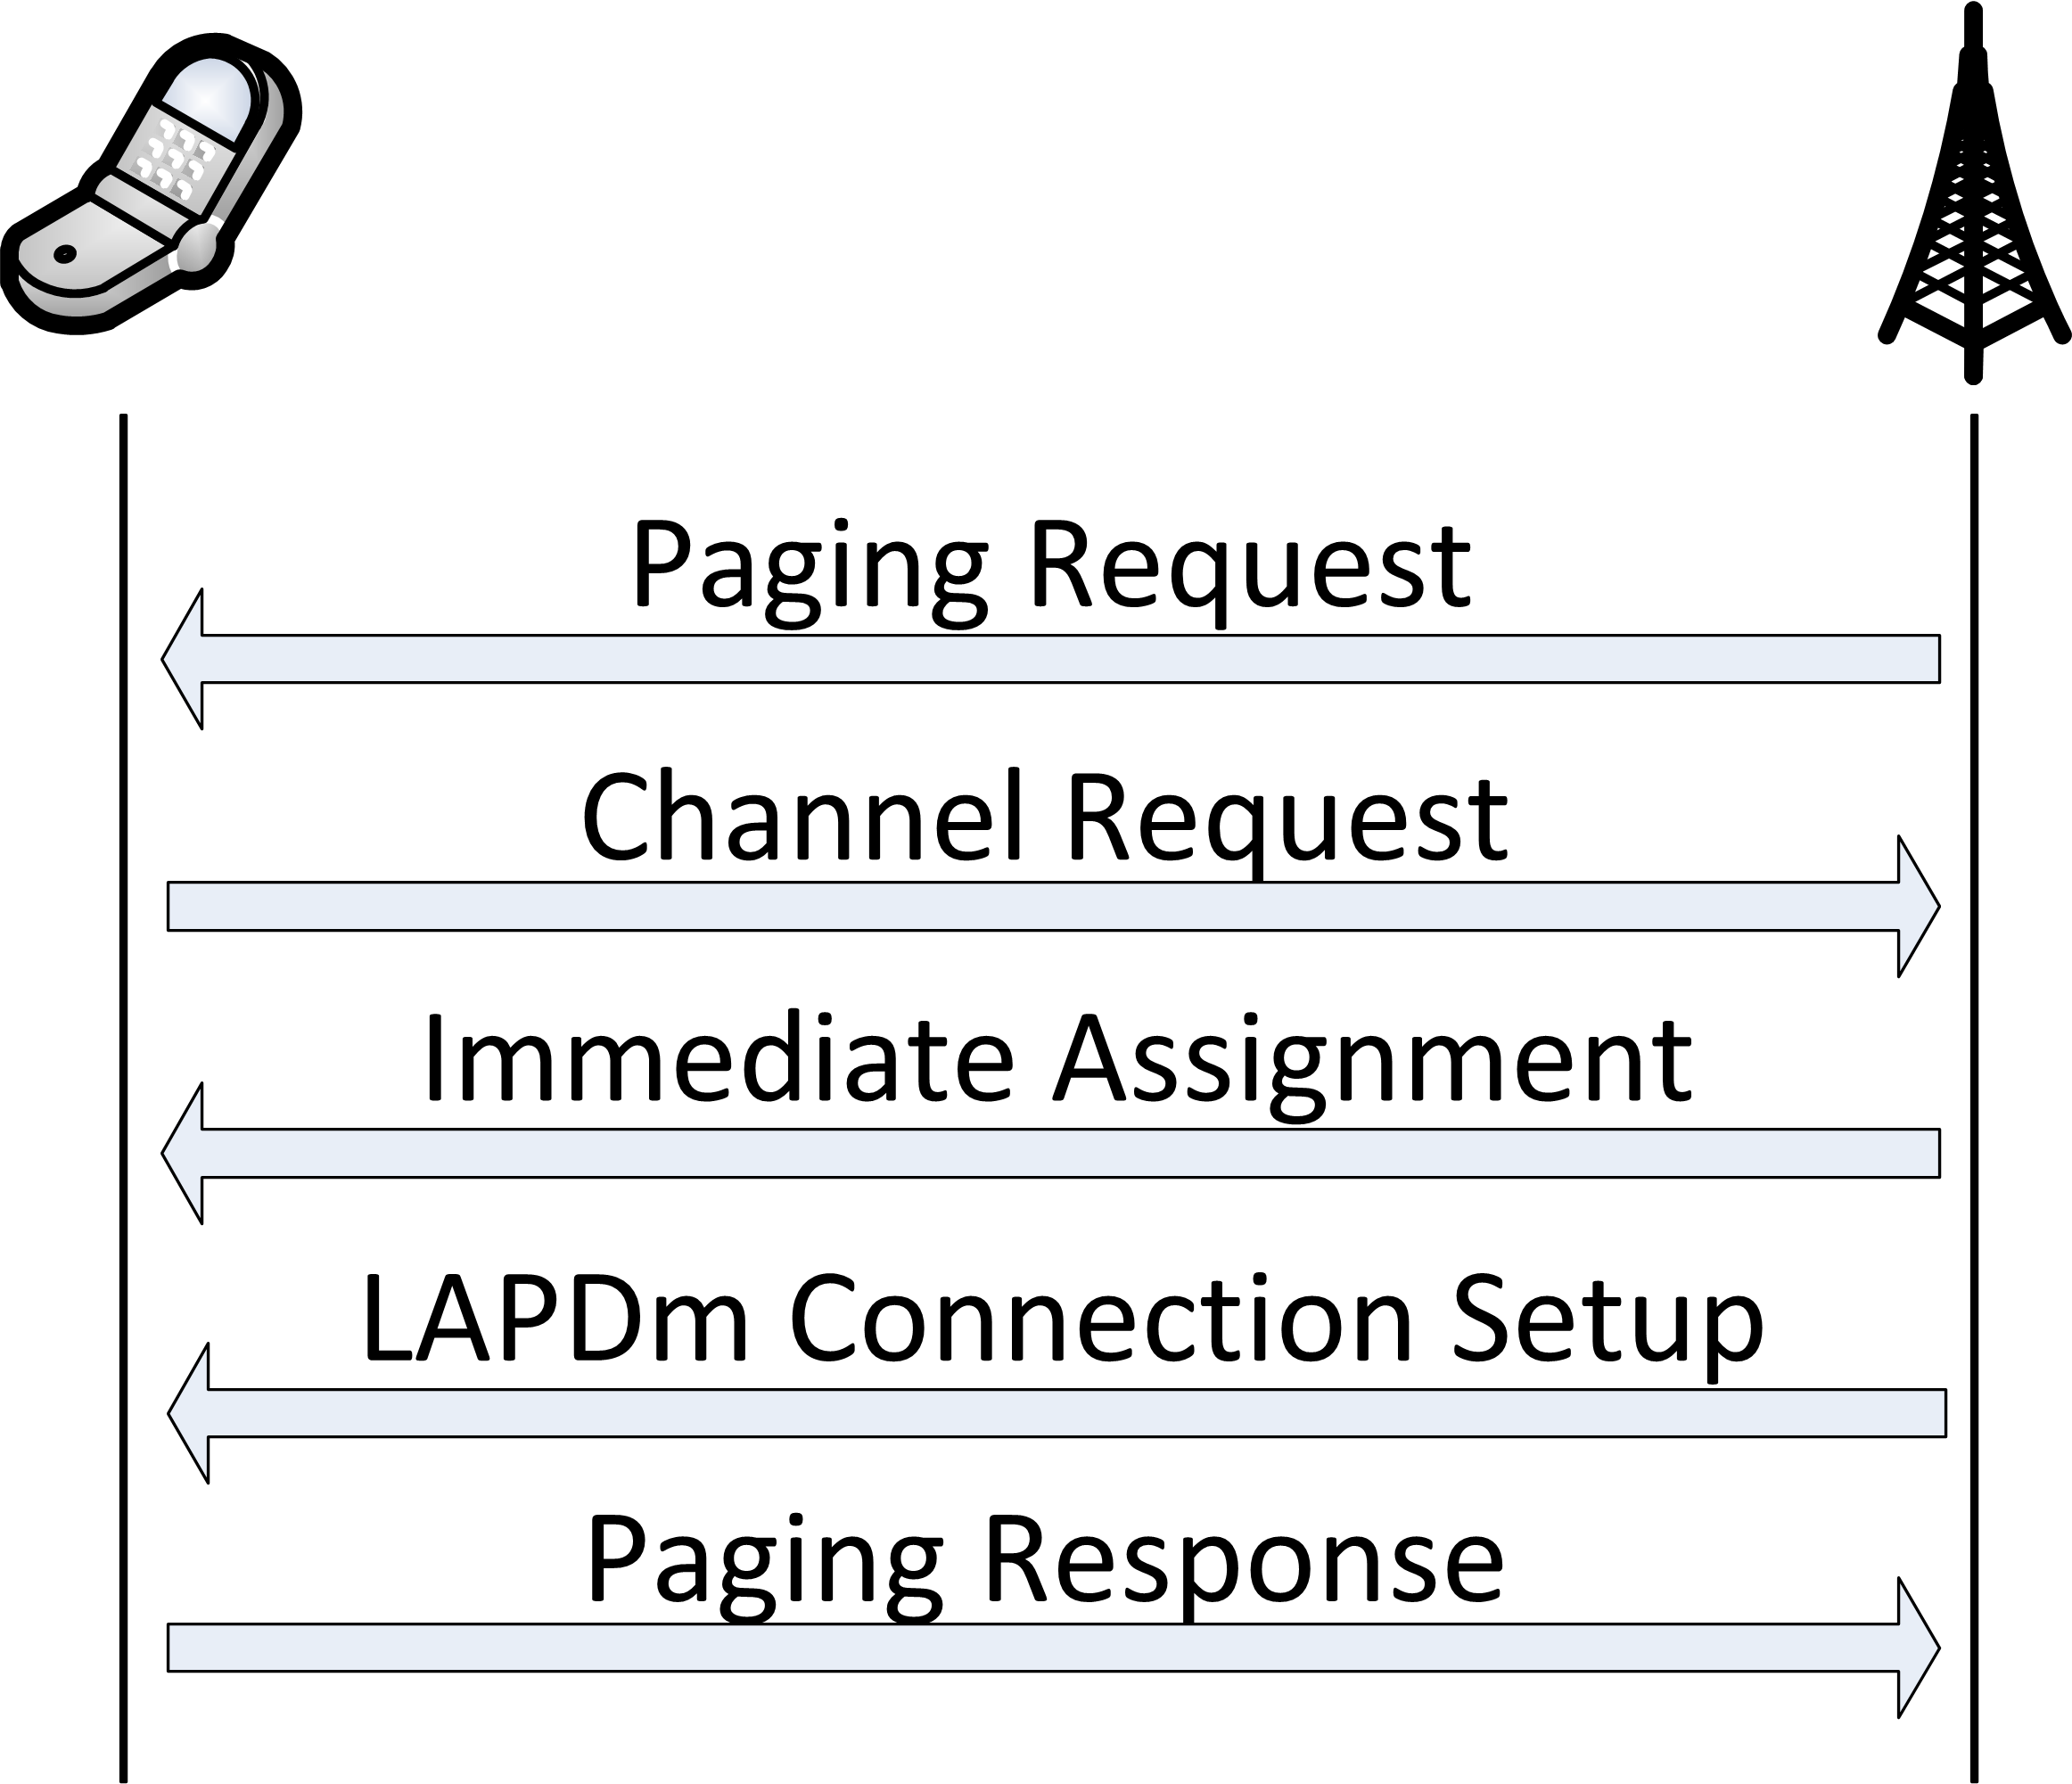
\includegraphics{../Images/Paging}
\caption{Procedure taken when the network has a call/text waiting for a passive subscriber.}
\label{fig:paging}
\end{figure}
The procedure is outlined in Figure \ref{fig:paging}.
A paging request by the network is answered by the \gls{ms} by requesting a dedicated channel, which is assigned by the network in turn with an Immediate Assignment message.
From this point on the connection can be set up.

An IMSI catcher however is not part of a provider's network, it is merely a proxy for a base station.
At best it can route calls into a network but it cannot take calls that are intended for a subscriber and route them.
Therefore an IMSI catcher will not page connected subscribers while a normal base station will have a very high number of pagings depending on the number of subscribers that are connected.
This is a significant difference between a catcher and a regular base station.
Since the \gls{pch} can be accessed publicly the \gls{icds} can use it as a source for information.
The \gls{pch} scan feature uses this finding, it tunes in to the \gls{pch} of a particular base station and scans the channel for a given amount of time, watching out for subscribers being paged and assigned channels.

This is an additional feature that can be used to identify an IMSI catcher.
It has not been implemented as a regular rule since each given base station needs some time to be scanned.
If that would be done on a regular basis for every station that has been discovered it would delay the whole scan by a large amount and the time difference between re-evaluations would be very high.
Therefore it was implemented as an extra feature to be used when needed.
The \gls{icds} also uses this method on particularly filtered base stations in User Mode as will be explained later.


\section{IMSI Catcher Detection System}
\label{sec:icds}
This section will discuss some technical aspects of the \gls{icds} software itself.
The first section focuses on architectural aspects and how the architecture can be extended whereas the second and third section will then explain how to configure and operate the application.

\subsection{Implemetation}
\begin{figure}
\centering
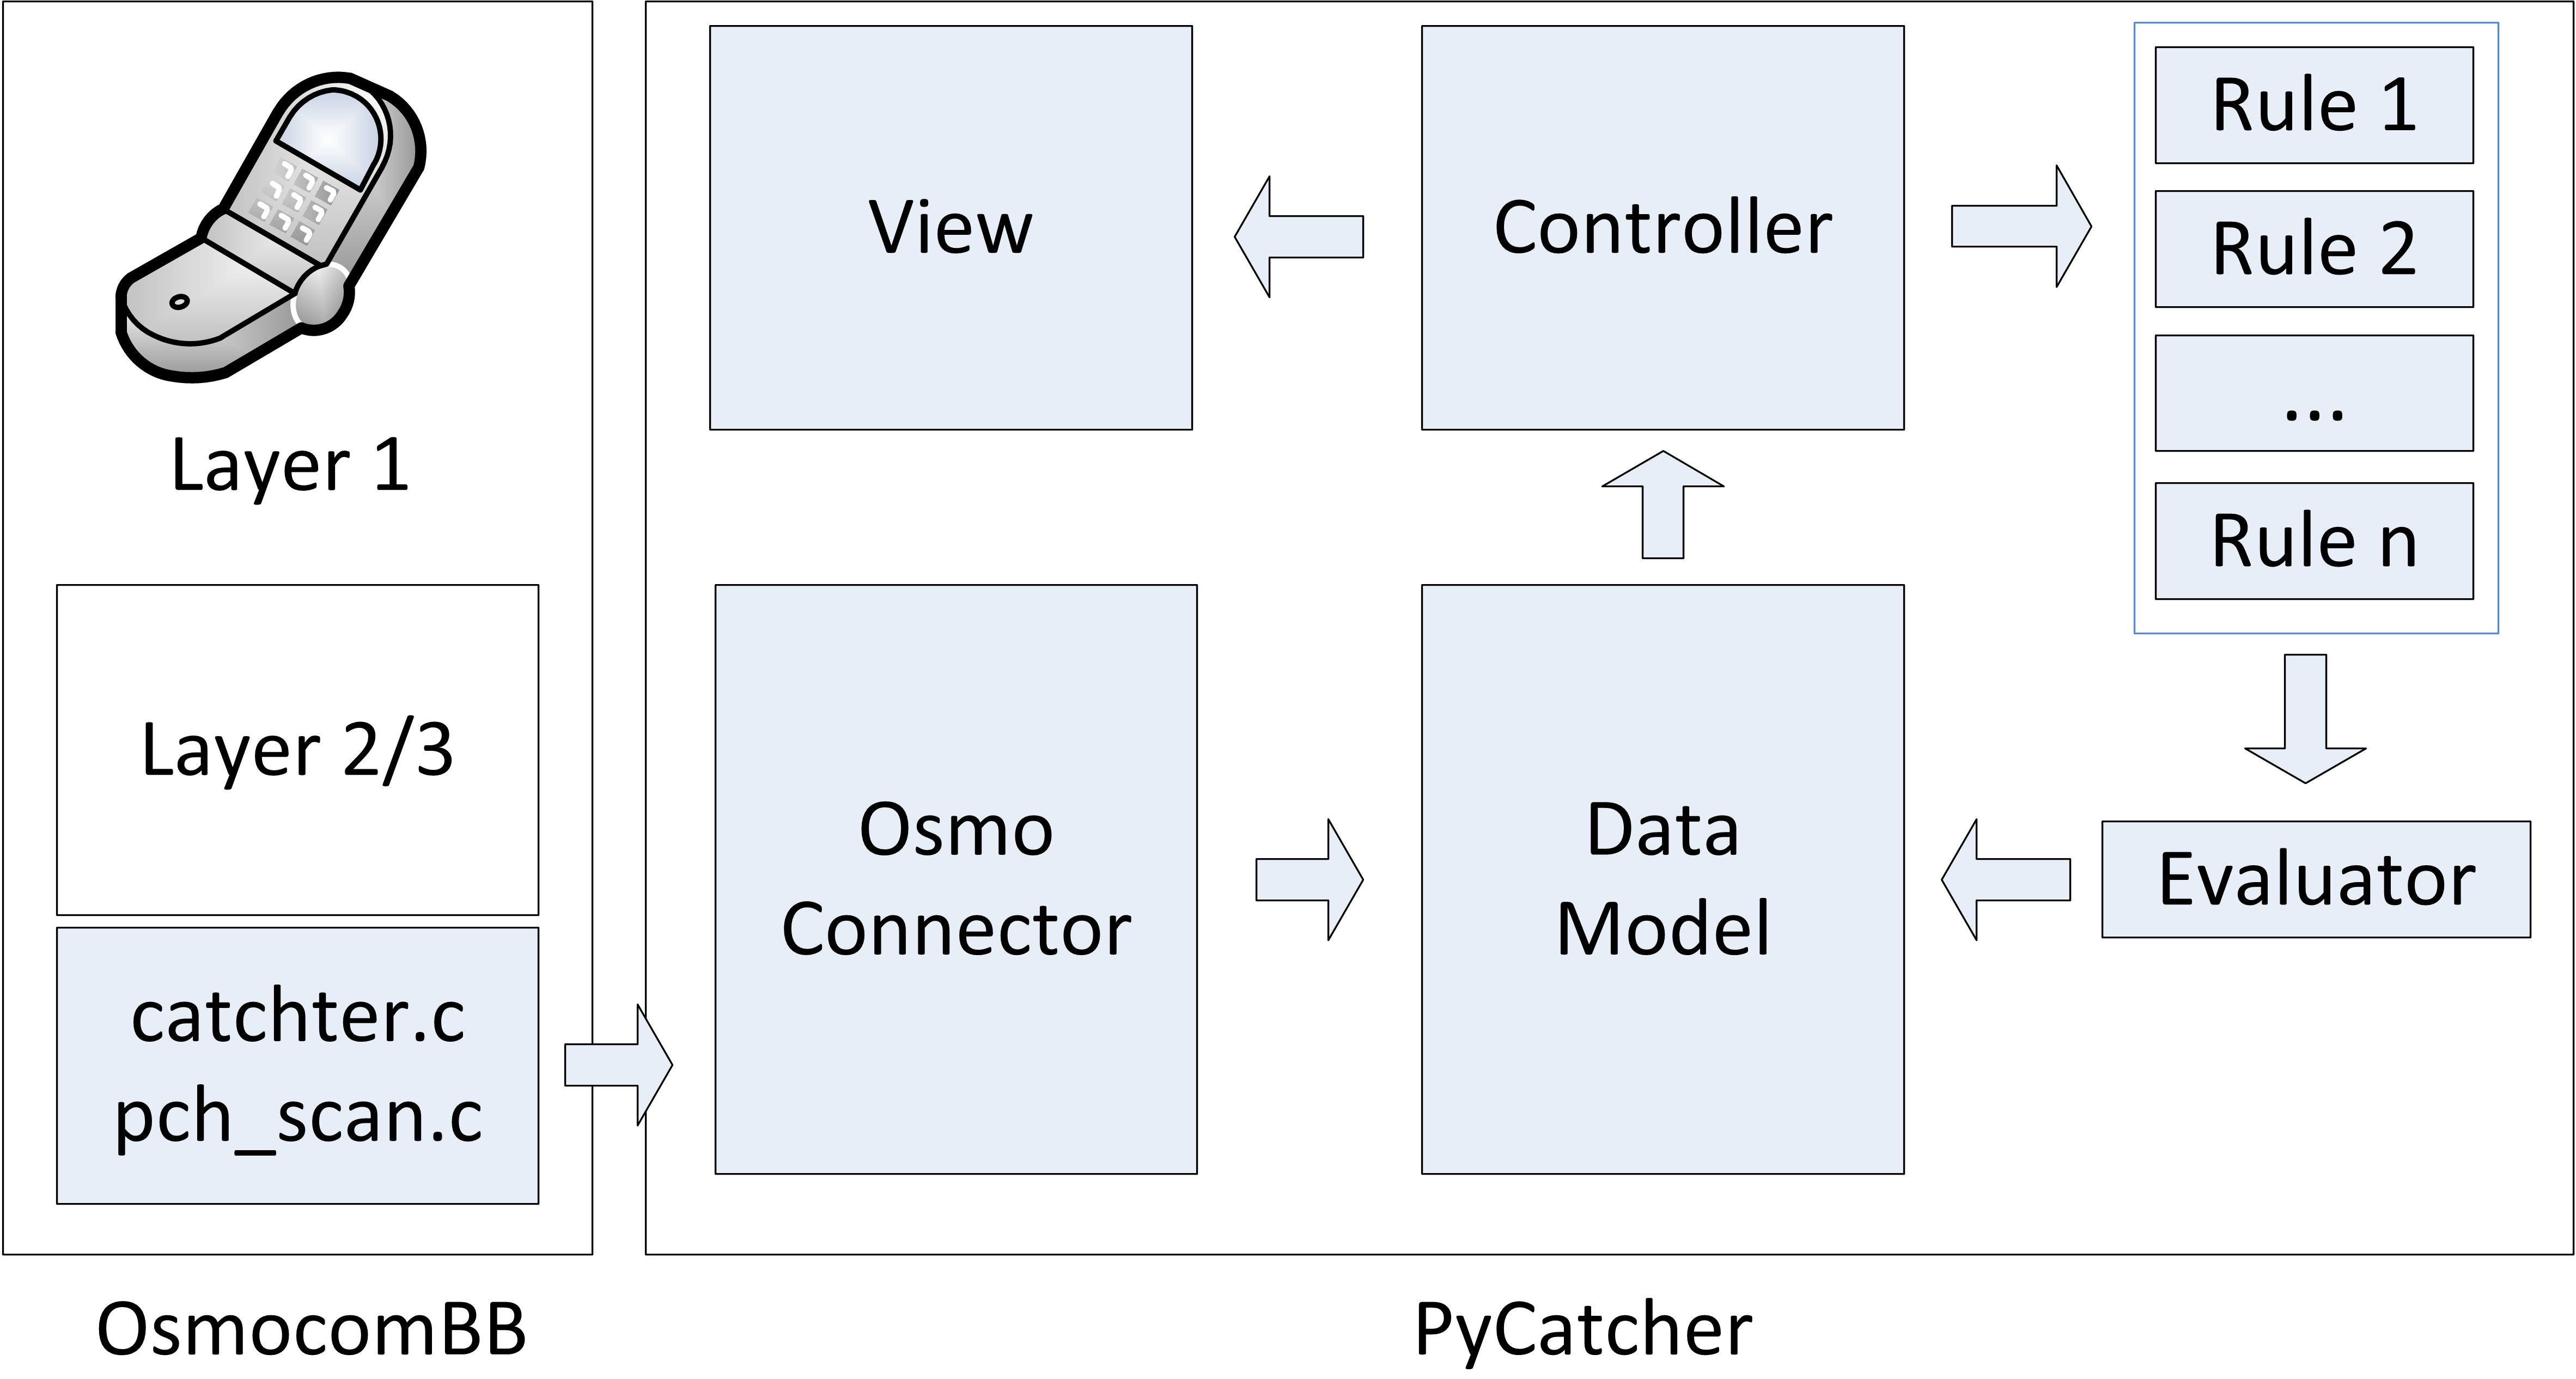
\includegraphics{../Images/Architecture_software}
\caption{System architecture of the ICDS. The arrows indicate the flow of data.}
\label{fig:architecture}
\end{figure}
Figure \ref{fig:architecture} shows a diagram describing the system architecture, the modules in light blue have been implemented for this project.
The application consists of two main parts.
One part, the \texttt{catcher}, is implemented inside the OscmocomBB framework, the other part, \texttt{PyCatcher}, is a Python application that uses \texttt{catcher} to harvest information and evaluate it afterwards.
Since the way \texttt{catcher} works has already been described in Section \ref{sec:info_gathering} this section will focus on the Python application part.

As mentioned before layer 1 of the \gls{gsm} stack is implemented in the firmware running on the Motorola C123.
Layer 2 and 3 are implemented on the computer and are used by the \texttt{catcher} software to harvest information from the \gls{bcch}.

The \texttt{PyCatcher} application was designed with a \gls{mvc} approach in mind to make it easy to implement new functionality.
The \gls{mvc} pattern is used to separate the data model of an application from the logic as well as from the way it is presented to the user.
That way each of the different components can be exchanged without affecting the other two.
An additional module has been added, the \texttt{OsmoConnector} that is loaded by the controller and spawns \texttt{catcher} as a child process.
It takes the output back in and transforms it into an object oriented representation of the discovered base stations.
These are then handed over and update the data model.
This way it can be ensured that only coherent and complete information is incorporated in the data model.
Another benefit is that the parsing module is isolated from the main program logic.

The \texttt{Controller} is the main part of the program and instantiates all the other modules.
It loads data from the model, triggers the evaluation and sends the results to the view to be displayed.
As discussed before there are several rules that can be evaluated for each base station.
These rules are stored within the controller and can be enabled or disabled by using the view that relays new rule configurations back to the controller to be applied. 
Whenever a new evaluation is requested the controller evaluates the active rules and gives the results to the active evaluator, afterwards the results are send to the view for display to the user.
Note that all the structures used are view independent, this way the current view could easily be exchanged with a web interface for example.

The \texttt{View} in this project consists of a GTK3 window with several forms for user input.
It is bound to the controller using PyGTK.
Details on the \texttt{View} and how to use it will be explained in Section \ref{sec:icds_operation}.

Rules and Evaluators were designed in a plugin fashion, since these are the main points where the program can be enhanced and new ideas can be realised.
Implementing a new rule or a new evaluator works by extending the rule or evaluator base class and implementing one method inside that derived class that contains the actual logic.
After that they only need to be added to the list of included evaluators and rules inside the \texttt{Controller}.
Appendix \ref{sec:extensions} gives an example of how this can be done.

\subsection{Configuration}
\label{sec:configuration}
\begin{figure}
\begin{lstlisting}
dictionary = {
	"key_1": value_1,		#single value
	"key_2": [value_2,value_3]	#value range
}
\end{lstlisting}
\caption{Configuration Dictionary in the settings file.}
\label{fig:python_dict}
\end{figure}
The configuration of the system is done in the file \texttt{settings.py}.
All configuration is done with python dictionaries, where each module has its own dictionary inside which it can have an arbitrary number of parameters with their respective values.
Figure \ref{fig:python_dict} shows an example with the two common cases used for parameters in this project.

The file consists of three main sections.
The first one contains parameters that are needed for the correct operation of the \gls{icds} system and have to be edited:
\begin{itemize}
	\item \texttt{Device\_settings}: The setting for the mobile phone that is used.
	In case the Motorola C123 is used, this section does not need to be edited.
	\item \texttt{Osmocom\_lib}: The path to the folder that contains the OsmocomBB framework.
	\item \texttt{Commands}: This is only to be edited when a newer version of the framework is used and the folder structure has changed since the release used in this project.s
\end{itemize}
The second and last sections are parameters for the different rules and evaluators.
A completely documented configuration file with all the rules and evaluator parameters can be found in Appendix \ref{sec:example_config}.
The file is read in as a python file.
This way python code can also be used to change settings dynamically depending on the environment or how the \gls{icds} is started.

\subsection{Operation}
\label{sec:icds_operation}
The \gls{icds} main application has to be started with root privileges since it needs to work with Unix sockets and open up connections to the Motorola C123.
This should be done by starting up the \texttt{main} class that initialises everything else.
\begin{lstlisting}
sudo python /path-to-project/Src/PyCatcher/src/main.py
\end{lstlisting}
After a brief loading time the main window shown in Figure \ref{fig:icds} should appear if a valid configuration is set up.

\begin{figure}
\centering
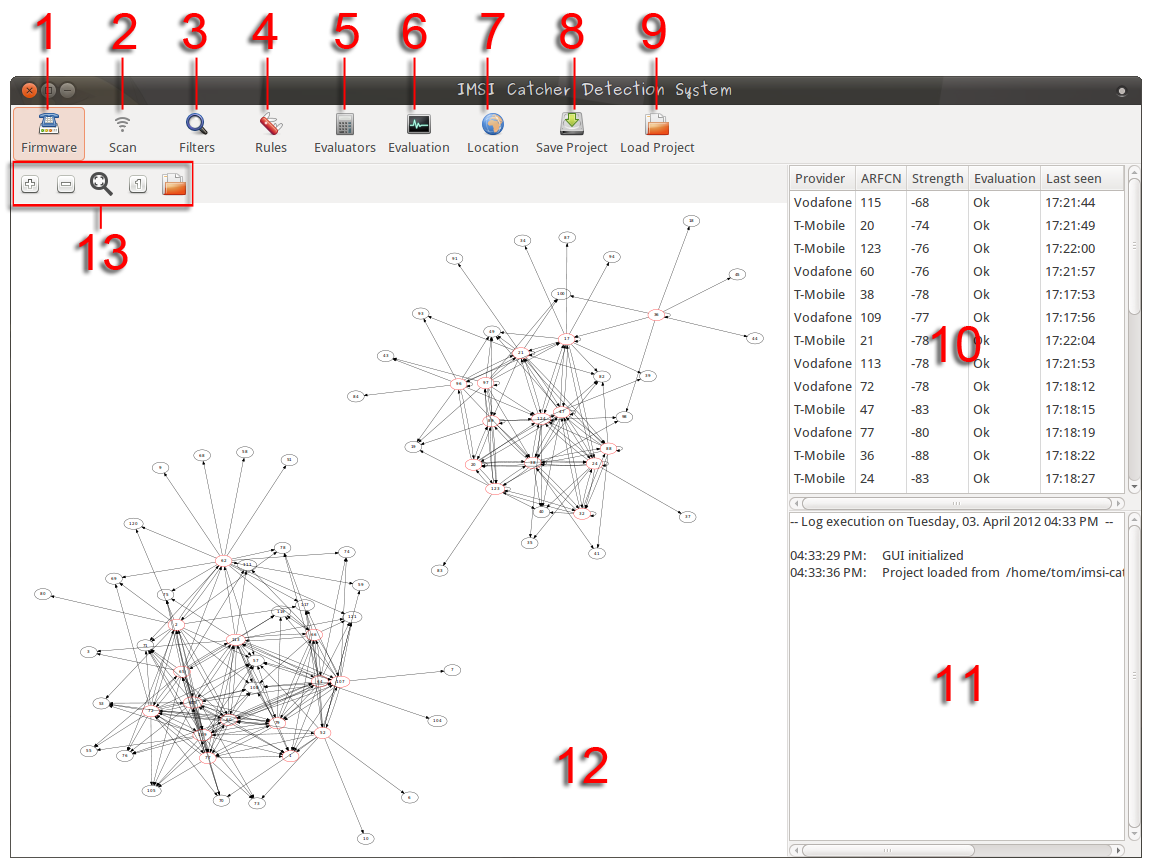
\includegraphics[width=\textwidth]{../Images/ICDS}
\caption{The ICDS main window.}
\label{fig:icds}
\end{figure}

The different elements shown in the main window are:
\begin{enumerate}
\item Firmware Loader: This button is used to load the OsmoconBB firmware onto the Motorola C123. 
For this to work, the mobile phone must be connected correctly to the computer and available on the configured \texttt{tty} interface.
After pressing the button on-screen instructions will lead the user through the process of flashing.

\item Scanner: This starts the \texttt{catcher} subprocess in the background and fills the data model with information on the discovered base stations.
During this process the Base Station List (11) and the Base Station Graph (13) will also be populated in realtime.
Re-evaluation on all base stations is done for every new \gls{bts} that has been found.

\item Filter Window: This brings up the window shown in Figure \ref{fig:filters_window}, where different view filters for the Base Station List and the Base Station Graph can be set.
Note that these filters do not modify the underlying data model or the behaviour of the scanner, the manipulate merely the view.
Hidden base stations will be scanned and added to the data model independent from the filters set, so they can be viewed at a later point if necessary.
Available filters are:
	\begin{itemize}
	\item Provider Filter: Takes a comma separated white list of providers that should be shown.
	\item ARFCN Filter: Takes a range of \glspl{arfcn} to be shown.
	\end{itemize}
These two filters can arbitrarily be combined together.
Filters are designed the same way as rules and evaluators, a new filter can be implemented by derivation of the base class.

\item Rules Window: All the rules implemented inside the \gls{icds} will be brought up with a check box to enable or disable these rules.
Disabling means that they will not be considered for the evaluation of a base station.
A screenshot can be seen in Figure \ref{fig:rules_window}.

\item Evaluator Window: This window will let the user choose  which evaluator to use for \gls{bts} evaluation.
Choosing a new evaluator will also trigger a re-evaluation of all the data collected so far.

\item Evaluation: This button brings up a separate window showing only the final evaluation of the scan.
The final evaluation shown in this dialog \emph{will} be affected by the filters set.
Base stations that are filtered out are not considered.

\item Databases Window: The window shown in Figure \ref{fig:databases} contains settings for all the databases the \gls{icds} uses.
These settings are mandatory if the Local Area Database Rule or the CellID Rule is going to be used.
It is also possible here to export the current scan as a \gls{csv} file or sqlite database to be used in other programs.

\item Encryption Window: This button brings up a dialog in which an \gls{arfcn} or a list of \glspl{arfcn} can be scanned to discover which encryption is used by the \gls{bts}.
A timeout for this operation can also be set here.
The longer the timeout the more likely another subscriber will connect to the base station in the given time frame.

\item Save/Load Project: The current state of the application can be saved as or loaded from a \texttt{.cpf} file.
This enables the user to continue a scan at a later time or to compare different data sets scanned at different points in time or locations with one another.

\item User Mode: The \gls{icds} is ultimately meant to be a tool that can be used by end users to check whether it is safe to initiate a phone call or not.
This dialog presents a way the already configured tool could be presented to end users.
Only the provider is to be entered and a final evaluation will be returned once the \gls{icds} is done with the process.

\item Base Station List: This list gives an overview of which base stations have been discovered so far along with some distinguishing information including its evaluation.
A detailed view of a base station can be brought up by selecting it in the list and pressing the enter or return key.
The report is separated into four main parts, the first being all the harvested parameters, followed by findings the different rules and evaluators yielded and a section with the raw uninterpreted system information data.
 
\item Log Window: Every important event inside the \gls{icds} is reported in the log together with a time stamp when it occurred.

\item Base Station Graph: This graph displays the base station found in the Base Station List (11).
A node represents a single \gls{bts} and is labelled with its respective \gls{arfcn}.
An edge from note $A$ to $B$ is drawn if node $B$ occurs in the Neighbouring Cells List of $A$.
Nodes with a white background have only been found inside Neighbouring Cell Lists but not yet by the \gls{icds} scanner itself whereas nodes with a red, yellow or green background have been found and evaluated with the colour representing either a critical, a warning or an ok status respectively.

\item Graph Controls: These are meant to make navigating the graph a bit easier.
From left to right the functionality is zoom in, zoom out, fit the whole graph to the viewport and display the graph in original size.
Zooming can also be done with the mouse wheel and it is possible to drag the graph around by clicking and holding it with the mouse and then moving it in the desired direction.
\end{enumerate}
\begin{figure}
\centering
\subfigure[Filters window.]{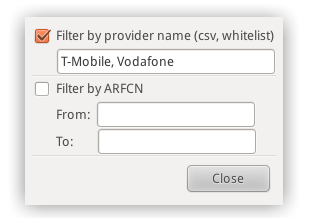
\includegraphics[width=.4\textwidth]{../Images/filter_window}\label{fig:filters_window}}
\subfigure[Rules window.]{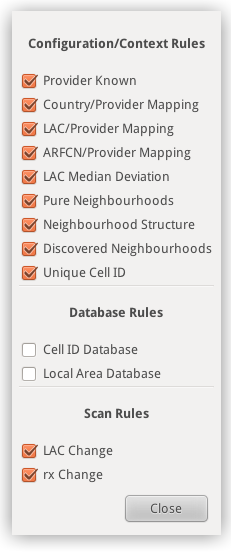
\includegraphics[width=.4\textwidth]{../Images/rules_window}\label{fig:rules_window}}\\
\subfigure[Databases window.]{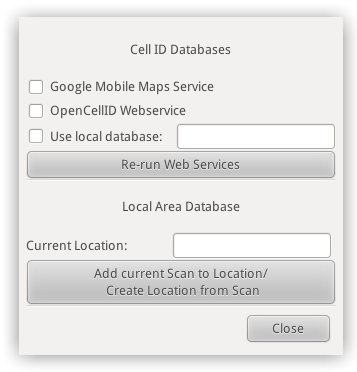
\includegraphics[width=.4\textwidth]{../Images/databases}\label{fig:databases}}
\subfigure[Encryption window (not yet implemented).]{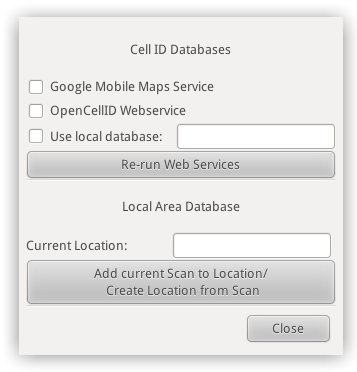
\includegraphics[width=.4\textwidth]{../Images/databases}\label{fig:encryption_window}}
\caption{Dialogs for different settings.}
\end{figure}
The procedure of operation differs depending on the purpose.

\paragraph{Sweep scans:} This is the normal mode of operation, scanning and evaluating all base stations in the perimeter.
This is also used for gathering various kinds of information to be used for analysis later.
At first the firmware needs to be flashed onto the device by pressing (1).
After the flashing process is finished the scan can be started by pressing (2).
Either before or during the scan (3),(4) and (5) can be used to customise the output or rules that should be considered during evaluation.
The scan can be stopped at any time.
Resuming the scan will renew the information in the Base Station List.
The scan will continue renewing information until it is terminated by the user.
The number of times a specific \gls{bts} has been scanned is shown in the \emph{Sightings} column of the Base Station List.

\paragraph{CellID Information:} CellID information can be obtained through several different means.
The Databases window shown in Figure \ref{fig:databases} can be brought up by pressing (7).
In the upper part settings concerning the acquisition of CellIDs can be found.
The operator has the choice between three different methods which can also be used in combination.
\emph{Google Mobile Maps Service} compares the station's CellIDs and \glspl{lai} to the ones in the Google database.
If they are found they are marked as such and additionally their location information will be set.
\emph{OpenCellID Web Service} performs the same task if activated.
As of now OpenCellID has a very low coverage compared to Google's service but it has been included since it is an open source approach that is actively developed and updated constantly.
The \emph{Use Local Databse} feature allows to use a previously build Location Area Database as CellID Database for lookups.
For this purpose the location to be used as database has to be entered in the textfield.
Offline lookups can be done that way, which are considerably faster that online lookups, the raw data used by the OpenCellID project can also be downloaded and used as a offline version for reference that way.
Since these lookups take some time if performed using webservices, this is not done while the scan is taking place, to not delay the acquisition of information from new base stations.
Pressing the button below the checkboxes will add the CellID Database information from the selected sources to all the stations currently in the base station list.
If more than one service is activated lookups will be done starting with the Google service, if active and using the next one in line only if the previous lookup failed.
Having at least one service activated and run on the base station list is a precondition for the CellID Rule to work.

\paragraph{Location Area Database:} Having set up the correct location in the \emph{Current Location} field of the databases window and having a valid database for that location are preconditions for the Location Are Database Rule to work.
To build up a database for a specific location a sweep scan for this location has to be done.
After the sweep scan is finished, the current location has to be set in the dialog and the button for adding/updating the database has to be pressed.
If there was no existing database for that location it will be created, otherwise the database will be updated with the new information acquired by the sweep scan.
To raise the quality of a Location Area Database it is recommended to do multiple sweep scans and integrate them rather than to only rely on a single scan.
This raises the probability that all \gls{bts} in the perimeter are found is higher and it solidifies the interval in which the base station signal strength varies.

\paragraph{PCH Scan:} A \gls{pch} scan can be conducted in addition to a sweep scan or as a standalone method therefore no scan data needs to be present.
If scan data is present however this feature will automatically augment the present data with its findings.
The first parameter is a comma separated list of \glspl{arfcn} that will be scanned.
The second parameter is the timeout. 
A scan for a particular \gls{arfcn} will tune in on the \gls{pch} of each \gls{arfcn} given and wait there until the timeout is reached gathering all paging messages that occur during the time period.
In the lower part of the dialog, after the scan has finished, a number will be given for each base station of how many pagings occured on average in five seconds.

\paragraph{User Mode:} Data needs to be present inside the \gls{icds} either by loading a project file for the corresponding location the system is used in or by having performed a sweep scan in advance.
There is only one input field in the dialog as Figure \ref{fig:user_mode} illustrates.
The user has to enter the provider name in this field and push the \emph{Start Evaluation} button.
From the scan data, the \gls{icds} extracts the base station with the highest reception for the given provider since this would be the station a \gls{ms} would connect to if started up.
It then performs a \gls{pch} scan on that station and accumulates the results from this additional scan with the data from the sweeps scan in a conservative manner.
Timeouts and retry attempts are taken from the \gls{pch} scan dialog.
Any adjustment made there will carry over in User Mode.

After the evaluation has been completed, the picture on the bottom will change to reflect the result found.

\section{Related Projects}
IMSI catcher detection is a topic that has not emerged until recently therefore not a lot of work and research has been done upon that topic.
This is mainly due to the fact that is was very hard to get information from the mobile network onto a computer for evaluation.
A fact that changed, or to be exact is now more accessible due to the OsmocomBB framework.

About the same time as this project, in December 2011, another project was announced with the same goals of detecting an IMSI catcher.
The project is called 'Catcher Catcher'\footnote{Catcher Catcher Wiki, \url{http://opensource.srlabs.de/projects/catcher/wiki/Tutorial} [Online; Accessed 05.2012]} and also builds up on the OsmocomBB framework.
The goals are the same however the means are very different.
As a codebase 'Catcher Catcher' uses the \texttt{mobile} application, a software that implements the firmware part of a mobile phone.
This results in an active approach to IMSI catcher detection.
An active connection is established between the phone and the base station in question.
One could say they try to identify the catcher by letting a bait phone get caught by it.

The advantage compared to the passive approach this project uses is that one has more sure means at hand of identifying a potential catcher.
Features that are already implemented are\cite{catcher_catcher}:
\begin{itemize}
	\item Encryption: Check whether encryption is enabled when doing a phone call.
	\item IMEI: \gls{imei} is not requested in Cipher Mode Complete message.
	\item LAC: \gls{lac} of a base station changes.
	\item Location Updates: IMEI is requested during Location Updates.
	\item Silent Text: Checks whether a silent text message is received.
	\item Call Setup: Do not receive a Call Setup message while being on a traffic channel for two seconds.
\end{itemize}
As one can see, missing encryption and reception of a silent text message are very strong indicators of being connected to a catcher.
This however comes at the cost of being discovered oneself.
Additionally if the IMSI catcher is configured only to allow specific IMSI numbers an active approach cannot be used to evaluate it.
A list of all the features that are planned can be found in Appendix \ref{sec:catcher_features}.

It is not clear whether the project has been abandoned since December 2012 or whether it is developed further. 
Activity on the wiki has seized after December 2012.